\chapter{Reading the figures and tables}
\label{ch:reading-the-figures}
\begingroup\sloppy

This chapter takes every figure and every table of the paper in turn and says what is
plotted, what the axes and units are, how to read the panel, which claim it supports,
and which registered experiment and generator produced it. The figures are reproduced
at text width from the paper's own files; the tables are described rather than
reproduced, because their entries are measured numbers that live in the paper's
generated fragments and nowhere else (\Cref{ch:protocol}). Figure and table numbers
refer to the draft of 20 September 2026 and follow the order of the captions in the
source; the file names do not change when the numbering does, so the file name is the
reliable handle.

\section{Conventions shared by every figure}
\label{sec:fig-conventions}

Four conventions recur, and a reader who has them in mind can read any panel of the
paper quickly.

\paragraph{The estimand.} Unless a caption says otherwise, an ``error'' is the
schedule-pooled relative score error of \Cref{ch:experimental-statistics}: squared score
error and reference score energy are summed over the twelve levels and over all sites of
all test sequences before the square root. It is dimensionless; zero is the exact
score; the isotropic score $-\vx$ sits near two thirds and the LMMSE floor of the
Laplace chain near one sixth (the paper's oracle table gives the values). A
\emph{per-level} error is the same ratio at one level.

\paragraph{Log axes.} Errors and information are plotted on logarithmic axes because
the theory is about exponential rates: a decay $e^{-ct}$ is a straight line of slope
$-c$ against a linear $t$ axis and a curve against a logarithmic one; the theory figure
uses log--log axes so that both the low-$t$ plateau and the high-$t$ power-law approach
are visible. A guide line labelled $e^{-4t}$ is drawn to be compared in slope, not in
level.

\paragraph{Seeds, bands and intervals.} Points are single fits; a line through them is
a mean or an RMSE over seeds; a shaded band is the range over replicates; an error bar
is a standard error over seeds or a percentile bootstrap interval; a paired ratio is
formed within seed before averaging (\Cref{ch:experimental-statistics}). Which of these
a panel shows is stated in its caption.

\begin{example}[Reading a rate and a crossover off a panel, by hand]
\label{ex:reading-slopes}
In panel (b) of the theory figure the two guide lines run from $t=1.2$ to $t=3$. Over
that interval a law $e^{-4t}$ falls by the factor $e^{-4\cdot1.8}=e^{-7.2}\approx7.5\times10^{-4}$,
that is by $7.2/\ln10\approx3.1$ decades, and a law $e^{-8t}$ by $6.3$ decades. A measured
curve that drops by six decades over the same interval has an average log-slope of
$-6\ln10/1.8\approx-7.7$, and one that drops by three decades has $-3.8$: the two guides
are three decades apart in their fall, which is what makes the two coordinates
distinguishable by eye. The crossover tick in panel (a) is at
$\tstar=\tfrac12\log\lmax(\Sig_0)$; the Toeplitz bound $\lmax\le(1+\corr)/(1-\corr)$ gives,
at $\corr=0.85$, $\lmax\le1.85/0.15\approx12.3$ and $\tstar\le\tfrac12\ln12.3\approx1.26$,
and the finite chain's value is a little lower. Either way the tick falls between the
ninth and tenth levels of the schedule ($0.98$ and $1.42$, \Cref{ch:protocol}), which is
where the learning figure shows the correlation being lost.
\end{example}

\paragraph{House style.} Every figure is drawn by a generator under \code{tools/} with
\code{tools/figstyle.py}: the text font is the paper's serif, mathematics is set by the
math engine, no prose is allowed inside a panel (only axis labels, tick labels, legend
entries and short series labels), a marked or excluded datum is a distinct glyph
explained in the caption, and a single-column figure is generated at column width and a
full-width one at text width. The rules are in \code{docs/FIGURE\_TABLE\_STANDARDS.md}
and two of them are enforced by the code.

\section{Figure 1: the mechanism (\code{fig\_mechanism.tex})}
\label{sec:fig-mechanism}

\providecolor{fgblue}{HTML}{2A78D6}
\providecolor{fgink}{HTML}{52514E}
\providecolor{fgmuted}{HTML}{8A8985}
\providecolor{fgfill}{HTML}{E1E0DC}
\begin{center}
%% Figure 1: the mechanism. Clean chain -> coordinatewise OU noising -> posterior stays a
%% chain (tree) -> two message sweeps -> Tweedie gives the exact score. TikZ, single column.
\begin{tikzpicture}[
  x=1cm, y=1cm, font=\footnotesize,
  lat/.style={circle, draw=black!70, fill=white, minimum size=4.2mm, inner sep=0pt},
  obs/.style={circle, draw=black!70, fill=black!15, minimum size=4.2mm, inner sep=0pt},
  fac/.style={rectangle, draw=black!70, fill=black!70, minimum size=1.8mm, inner sep=0pt},
  ufac/.style={rectangle, draw=black!70, fill=white, minimum size=1.8mm, inner sep=0pt},
  msg/.style={-{Latex[length=1.6mm]}, thick, draw=blue!70!black},
  lab/.style={text=black!60, font=\scriptsize},
]
  % latent chain
  \foreach \i in {1,...,5} {
    \node[lat] (a\i) at (1.15*\i, 1.2) {$a_{\i}$};
  }
  \foreach \i/\j in {1/2,2/3,3/4,4/5} {
    \node[fac] (k\i) at ($(a\i)!0.5!(a\j)$) {};
    \draw[black!70] (a\i) -- (k\i) -- (a\j);
  }
  \node[lab, anchor=east] at (0.55, 1.2) {$\kernel(a_{i}\!\mid\! a_{i-1})$};
  % unary factors and observations
  \foreach \i in {1,...,5} {
    \node[ufac] (l\i) at (1.15*\i, 0.6) {};
    \node[obs] (x\i) at (1.15*\i, 0.0) {$x_{\i}$};
    \draw[black!70] (a\i) -- (l\i) -- (x\i);
  }
  \node[lab, anchor=east] at (0.55, 0.6) {$\like(x_i\!\mid\! a_i)$};
  \node[lab, anchor=east] at (0.55, 0.0) {$\vx_t=e^{-t}\va+\sqrt{\Dt}\,\vz$};
  % messages
  \draw[msg] ($(a1)+(0,0.42)$) -- node[above, lab, yshift=-1pt] {$\lmsg$} ($(a3)+(-0.25,0.42)$);
  \draw[msg] ($(a5)+(0,0.42)$) -- node[above, lab, yshift=-1pt] {$\rmsg$} ($(a3)+(0.25,0.42)$);
  % annotation: no edges added, exact score
  \node[lab, anchor=north, text width=6.0cm, align=center] at (3.45, -0.45)
    {unary factors add no edges among the $a_i$: the posterior is the prior's chain, a tree;
     two sweeps give $\pmean{\va}$, and $\score(\vx,t)=-(\vx-e^{-t}\pmean{\va})/\Dt$ exactly};
\end{tikzpicture}

\end{center}

\paragraph{What is drawn.} A factor graph (\Cref{ch:factor-graphs-bp}) with three rows:
the latent sites $a_1,a_2,\dots,a_i,\dots,a_{\nsites}$ (white circles) joined by the
transition factors $\kernel(a_i\mid a_{i-1})$ (filled squares); one unary factor
$\like(x_i\mid a_i)$ per site (open squares); and the observed noised coordinates $x_i$
(shaded circles). Two blue arrows are the forward and backward messages $\lmsg$ and
$\rmsg$ meeting at the query site $i$. The interior is elided and the last site is
labelled symbolically, so the picture states the general case.

\paragraph{How to read it.} Follow any path between two latent variables: it runs along
the top row only. Conditioning on $\vx$ attaches the unary factors below each site and
adds no edge among the latent variables, so the posterior graph is the prior's chain, a
tree, and sum-product on it is exact. Where the two arrows meet, the product
$\lmsg_i\like\rmsg_i$ is the site marginal, whose mean is $\pmeansite{i}$, and Tweedie's
identity (\Cref{ch:ou-channel-tweedie}) turns that mean into the score.

\paragraph{Claim and source.} The claim is the first sentence of the paper: the score is
exact. There is no experiment behind the figure; it is a TikZ drawing whose palette is
the same as the plotted figures'.

\section{Figure 2: what survives diffusion noise (\code{fig\_theory.pdf})}
\label{sec:fig-theory}

\begin{center}
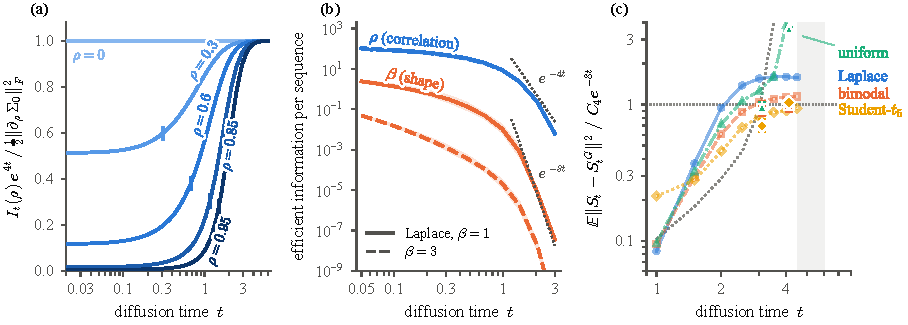
\includegraphics[width=\textwidth]{fig_theory.pdf}
\end{center}

\paragraph{Panel (a).} Horizontal axis: diffusion time $t$, logarithmic. Vertical
axis: the exact Fisher information of the Gaussian chain about $\corr$, divided by its
predicted asymptote $\tfrac12\Frob{\partial_\corr\Sig_0}^2e^{-4t}$, so that the theorem
predicts the value one (dotted line). One curve per correlation, in a blue ramp from
$\corr=0$ to $0.95$; the short vertical tick on each curve marks its crossover
$\tstar(\corr)=\tfrac12\log\lmax(\Sig_0)$. Reading: every curve rises to one, which is
the paper's Theorem~3 for a covariance coordinate, exactly (there is no Monte Carlo in
this panel; the information is the closed-form trace of
\Cref{ch:fisher-cramer-rao}); the more correlated the chain, the later the curve
arrives, and the tick shows that the arrival is governed by $\tstar$. At $\corr=0$ the
curve is one at every $t$. The curves are computed by the \code{gauss} part of E01.

\paragraph{Panel (b).} Both axes logarithmic: $t$ against the efficient Fisher information
per noised sequence, for the correlation coordinate $\corr$ (degree two, blue) and the
shape coordinate $\beta$ (degree four, orange) of the generalised-Gaussian chain, at the
Laplace member $\beta=1$ (solid) and at $\beta=3$ (dashed), estimated from
per-sequence scores obtained by Fisher's identity through the tree-exact recursion
(\Cref{ch:maximum-likelihood-em}); the bands are the range over eight replicates, and the
two dotted guides have slopes $-4$ and $-8$. Reading: above the crossover the two
families of curves run parallel to their guides, three decades apart, which is the
order-by-order decay; below it both are shallower, which is the pre-asymptotic regime.
The kinked Laplace density reaches the numerical floor of the outer-product estimate near
$t=2.5$, which is why the slopes quoted in the text are fitted on the smooth members.
The curves are the \code{shape} part of E01; the fitted slopes come from
\code{tools/make\_theory\_numbers.py}.

\paragraph{Panel (c).} Both axes logarithmic: $t$ from about one to five against the
measured closure gap $\E\lVert\score-\Sgauss\rVert^2$ divided by its predicted
value $\tfrac16\Frob{\kfour}^2e^{-8t}$, so that the theorem predicts one (dotted line).
Four innovation families (Laplace, bimodal, uniform, Student-$t_5$) from E18 on the wide
$(3201,32)$ grid: thin curves with small markers are the ratio from $512$ sequences,
paired across levels by a common noise draw, so their \emph{shape} is precise while
their level carries a common sampling factor; the bold markers with bars at $t=3$ and
$4$ are the constant from many more sequences with a chain bootstrap interval, and they
are what pins the level. The grey dotted curve is the same Student-$t_5$ sequences on the
operating $(801,8)$ domain, where the truncated prior drives the reference; the shaded
region beyond $t=4.5$ is where the double-precision floor of the posterior means enters.
Reading: every family reaches one within its interval, Student-$t_5$ included; the
departure of the grey curve is a truncation artefact, not the moment condition; the
uniform family, with the smallest constant, hits the floor first. Sources: E18 (the
\code{chain} and \code{constant} parts) and the E01 protocol; drawn by
\code{tools/make\_fig\_theory.py}.

\paragraph{Claims supported.} The rates $e^{-4t}$ and $e^{-8t}$, the constants
$\tfrac12\Frob{\partial_\corr\Sig_0}^2$ and $\tfrac16\Frob{\kfour}^2$, the crossover, and
the heavy-tailed regime as a statement about expectations rather than samples
(\Cref{ch:attenuation-theorems}).

\section{Figure 3: learning through noise (\code{fig\_learning.pdf})}
\label{sec:fig-learning}

\begin{center}
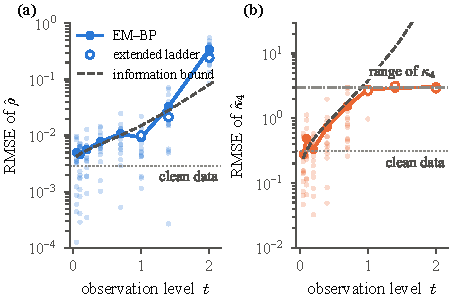
\includegraphics[width=\textwidth]{fig_learning.pdf}
\end{center}

\paragraph{What is plotted.} Two panels with a linear horizontal axis, the observation
level $t$ at which all $\nseq=512$ training sequences were noised, and a logarithmic
vertical axis. Panel (a): the error of the fitted correlation $\hat\corr$; panel (b):
the error of the fitted innovation excess kurtosis $\hat\kfour$. In each, faint points
are the sixteen individual fits $|\hat\theta-\theta|$ at that level, the solid line is
their RMSE, the dashed line is the Cram\'er--Rao reference $1/\sqrt{\nseq I_t}$ read from
the frozen E01 efficient information at the Laplace member (through the chain rule for
the kurtosis), the dotted horizontal line is the clean-data fit (the optimiser's own
floor at $t=0$), and in panel (b) the dash-dotted horizontal line at $3$ is the full range
of the coordinate, the distance from a Gaussian innovation to the truth. In the current
draft hollow markers add the same fits with the EM ladder extended (E06c), the budget
control (\Cref{ch:model-selection}).

\paragraph{How to read it.} At the lowest levels the points cluster around the reference
in both panels: the estimator is unimodal and at the information reference while the
coordinate is identifiable. Moving right in panel (b), the cloud splits into a cluster
near the reference and a group of points at the range line: those are fits that
collapsed to a Gaussian innovation. Where the dashed reference crosses the range line,
the information runs out and every fit collapses; panel (a) shows the correlation
surviving to a higher level, and being lost only past the crossover. The vertical
distance between the solid line and the dashed line, in decades, is the estimator's
inefficiency; where the points sit \emph{below} the reference the estimator is biased
(shrunk by early stopping) and the reference, being for an unbiased estimator in a
one-parameter family, is a yardstick rather than a bound (\Cref{ch:em-through-noise}).

\paragraph{Claims and sources.} The per-level statements of the paper's Section~4 (at
the reference while identifiable; collapse where the reference crosses the range; the
correlation survives to the crossover; the two highest levels possibly budget-limited).
Source: E06 (and E06c), \code{outputs/E06/levels.csv}; drawn and its macros written by
\code{tools/make\_learning\_numbers.py}; the collapse fractions and dispersions of the
text are from \code{tools/make\_audit\_numbers.py}. The moment estimators of E19
(\Cref{ch:quasi-likelihood-moments}) are quoted in the text as the rate-correct
competitor and, in the audit's recommended redesign, would appear as a second pair of
curves.

\section{Figure 4: capacity across the family (\code{fig\_family.pdf})}
\label{sec:fig-family}

\begin{center}
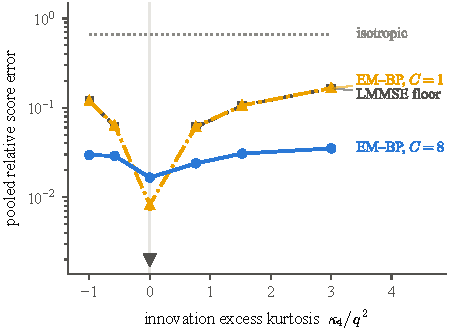
\includegraphics[width=\textwidth]{fig_family.pdf}
\end{center}

\paragraph{What is plotted.} Horizontal axis: the innovation's excess kurtosis
$\kfour/\ivar^2$, from $+3$ at the Laplace member through $0$ at the Gaussian member to
about $-1.1$ at the platykurtic end, along the generalised-Gaussian family at fixed
$\corr$ and variance; a vertical grid line marks zero. Vertical axis: pooled relative
score error, logarithmic. Four curves: the isotropic reference (grey dotted), the LMMSE
floor (dark dashed with hollow squares), EM--BP with a single Gaussian innovation
$\ncomp=1$ (dash-dotted triangles) and with $\ncomp=8$ (solid circles), the last two with
standard-error bars over sixteen seeds at $\nseq=512$. The floor is exactly zero at the
Gaussian member, which a logarithmic axis cannot show, so the dashed line is broken
there and a caret at the bottom marks the point.

\paragraph{How to read it.} The floor traces a V with its vertex at the Gaussian member:
that is the price of second-order closure across the family, largest where the fourth
cumulant is largest in either sign. The $\ncomp=1$ curve lies on the V within its bars
at every member, which is Proposition~1 read across a family
(\Cref{ch:gaussian-closure-lmmse,ch:quasi-likelihood-moments}). The $\ncomp=8$ curve
stays low throughout and meets the $\ncomp=1$ curve at the Gaussian member, where the
gap between them, the paired gain of capacity, is a small loss: with no fourth-order
structure to buy, the extra components only add variance.

\paragraph{Claims and sources.} Capacity buys exactly what closure discards; the gain is
ordered by $\kfour$; at the Gaussian member it reverses. Source: E02b,
\code{outputs/E02b/family.csv}; \code{tools/make\_family\_numbers.py}.

\section{Figure 5: where the structure stops helping (\code{fig\_misspec.pdf})}
\label{sec:fig-misspec}

\begin{center}
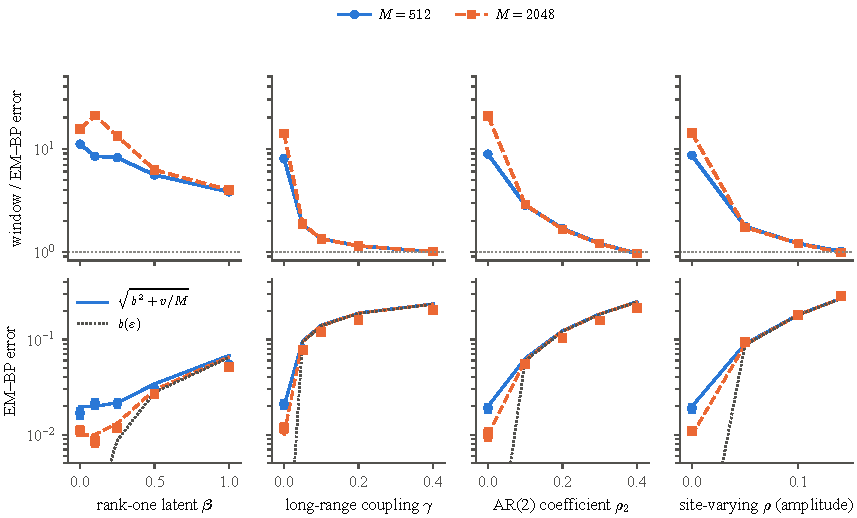
\includegraphics[width=\textwidth]{fig_misspec.pdf}
\end{center}

\paragraph{What is plotted.} Two rows of four panels, one column per misspecification
mechanism of \Cref{ch:misspecification-edgeworth}: the rank-one latent (strength
$\beta$), long-range precision coupling ($\gamma$), the AR(2) second coefficient
($\corr_2$) and the site-varying correlation (amplitude $\delta$). Top row: the ratio of
the radius-$2$ window head's error to EM--BP's, formed within seed and averaged,
against the strength, logarithmic vertical axis shared across the row, one curve per
sample size ($\nseq=512$ and $2048$; the legend is a single strip above the row); the
dotted horizontal line is ratio one. Bottom row: EM--BP's own error at both sizes
(points with paired standard errors), the closed-form bias $b(\varepsilon)$ of the
Kullback--Leibler projection (dark dotted) and the finite-sample prediction
$\sqrt{b(\varepsilon)^2+v/\nseq}$ for each size (lines), with $v$ read from the
well-specified cells.

\paragraph{How to read it.} In the top row, a curve above the dotted line means the
misspecified chain estimator still beats the network; where it crosses below, the
network wins. The crossing is reported as the two bracketing strengths, never as a
fitted point. A curve that stays above the line across the whole swept range (the
rank-one latent) is a mechanism this estimator absorbs; a curve that reaches the line
but does not cross it (long-range coupling, at the largest strength) is a tie. In the
bottom row the two sizes separate estimation from bias: at zero strength the points of
the two sizes are apart and the larger sample is lower (estimation); at large strength
they coincide on the dotted bias curve (bias that no sample size removes). The slope of
the bias curve at small strength on these axes is its order: linear for three mechanisms
and quadratic for the latent.

\paragraph{Claims and sources.} Graceful degradation; mechanism-dependent break-even;
the closed-form bias reproducing the large-sample error; the order in the strength
explaining which mechanisms bite. Sources: E08 (\code{outputs/E08/misspecification.csv})
for the points and ratios, E17 (\code{outputs/E17/bias.csv}) for the curves;
\code{tools/make\_misspec\_numbers.py}. The network arm is the radius-$2$, width-$64$
window head of \Cref{ch:neural-baselines}, not the screen's radius-$4$ winner.

\section{Figure 6: the floor across correlation (\code{fig\_phase.pdf})}
\label{sec:fig-phase}

\begin{center}
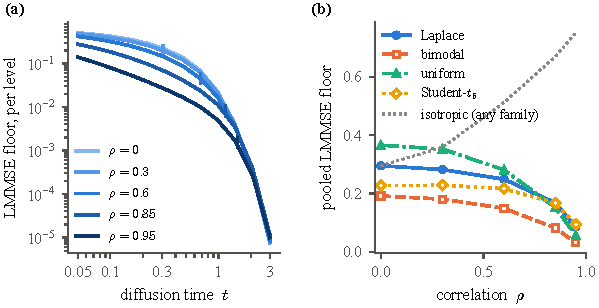
\includegraphics[width=\textwidth]{fig_phase.pdf}
\end{center}

\paragraph{What is plotted.} An appendix figure from the deterministic oracle ladder.
Panel (a): log--log axes, $t$ against the per-level LMMSE floor on the Laplace chain, one
curve per correlation in $\{0,0.3,0.6,0.85,0.95\}$ (blue ramp), with a tick at
$\tstar(\corr)$ on each. Panel (b): the schedule-pooled LMMSE floor against $\corr$
(linear horizontal axis) for the four non-Gaussian families, with the isotropic
reference as a grey dotted curve (the isotropic floor is the same for every family, so
one curve serves). In the current draft the Student-$t_5$ curve is computed on a wider
domain, where its $\corr=0$ cell is converged (E07b, E07c); earlier drafts ringed that
point as excluded.

\paragraph{How to read it.} In panel (a) each floor is flat at low $t$ and collapses after
its tick: past the crossover the twin's score is nearly the score, at every
correlation. In panel (b) the families are ordered by the size of their fourth
cumulant at every $\corr$ (Laplace above uniform above bimodal, with the heavy-tailed
family where its constant puts it), and every floor falls with $\corr$ while the
isotropic reference rises: a strongly correlated chain has a score dominated by its
second-order part, so closure costs relatively less and learning nothing costs more.

\paragraph{Claims and sources.} The floor is a function of the innovation law and of
$\corr$; the crossover locates its collapse; the ordering by $\kfour$. Source: E07 (and
E07b, E07c), \code{outputs/E07/ladder.csv}; \code{tools/make\_fig\_phase.py}, which also
writes the phase macros.

\section{Figure 7: locality against its floor (\code{fig\_locality.pdf})}
\label{sec:fig-locality}

\begin{center}
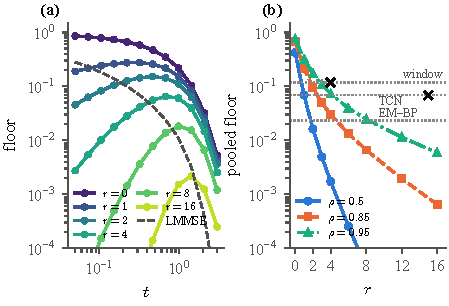
\includegraphics[width=\textwidth]{fig_locality.pdf}
\end{center}

\paragraph{What is plotted.} Panel (a): log--log axes, $t$ against the relative score
error of the best estimator that sees only the window $x_{i-r},\dots,x_{i+r}$ (the exact
posterior mean given the window, computed by sum-product on the sub-chain with the exact
marginal of the window's first site as initial factor), for radii $r\in\{0,1,2,4,8,16\}$
in a colour ramp, on the Laplace chain at $\corr=0.85$, with the Gaussian twin's full
LMMSE as a dashed line for scale. Panel (b): the same floor pooled over the schedule
against the radius, one curve per correlation in $\{0.5,0.85,0.95\}$; dotted horizontal
lines mark the frozen all-site errors at $\nseq=2048$ of the window head, the dilated
TCN and EM--BP, and crosses mark the two networks' radii.

\paragraph{How to read it.} In panel (a) the radius-zero curve is the price of using no
neighbours at all, and the curves fall quickly with $r$: at low noise one site is
nearly enough, at intermediate levels even a radius of sixteen leaves a small
remainder. In panel (b) the floor at the window head's radius is far below the head's
own error line: the plateau of the local architecture is not the information ceiling of
its radius but a limit of the architecture and its training. The gap between the floor
at $\corr=0.5$ and at $0.95$ shows that locality costs more when the chain is more
correlated, and that at $\corr=0.95$ the radius-four floor approaches the LMMSE floor
itself.

\paragraph{Claims and sources.} The withdrawal of ``locality is a ceiling'' and its
replacement by the floor; the non-Gaussian content of a wider window. Sources: E15
(\code{outputs/E15/locality.csv}) for the floors, E03 and E02a for the marks;
\code{tools/make\_fig\_locality.py}. One point to check against the paper: the
generator places the window head's cross at radius $2$ and the caption calls it the
radius-$2$ head, while the confirmatory head of E03, whose error the mark shows, has
radius $4$ (\code{outputs/E03/winners.json}); the text beside the figure compares that
error with the radius-$4$ floor.

\section{The tables}
\label{sec:tables}

\subsection{Table 1: capacity (\code{tab-capacity.tex})}

Rows: the LMMSE floor and EM--BP with $\ncomp\in\{1,2,4,8,16\}$. Columns: the four sample
sizes and a last column, $\nseq=\infty$, which is not a fit but the population reference
of E09: the $\ncomp$-component mixture innovation closest in Kullback--Leibler divergence
to the Laplace law, scored by tree-exact BP on the same test bundles. Entries are the
all-site pooled error averaged over sixteen seeds; standard errors, paired differences
and bootstrap intervals are in the macros and the text. A dagger marks a fit whose
narrowest component is under two grid cells, reported and not dropped. Reading: the
$\ncomp=1$ row equals the floor row to the printed precision at every size, which is the
apparatus check of \Cref{ch:quasi-likelihood-moments}; every $\ncomp\ge2$ row is far
below it; the best capacity moves right with the sample size; the $\infty$ column says
what each capacity could express with unlimited data, a reference and not a bound
(a Kullback--Leibler-optimal innovation need not minimise the score error). Sources:
E02a (\code{outputs/E02a/capacity.csv}) and E09 (\code{outputs/E09/floor.csv});
\code{tools/make\_capacity\_numbers.py}. The retired reading of the earlier capacity
study and its stopping-rule diagnosis are in the paper's appendix on capacity.

\subsection{Table 2: baselines under one recipe (\code{tab-baselines.tex})}

Rows: the four sample sizes. Columns: the isotropic reference, the LMMSE floor, the six
architectures (MLP, window head, TCN, bi-GRU, transformer, U-Net) under interface~A with
their screened configurations, and EM--BP with $\ncomp=8$. Entries: all-site pooled error,
mean over the sixteen confirmatory seeds, every arm on identical test bundles (the
oracles and EM--BP come from the capacity experiment and are joined on the bundle hash).
Reading: down a column, how each estimator improves with data; along a row, the ladder
isotropic, networks, floor, EM--BP, exact (zero). The fully connected network is far
behind the weight-shared ones at every size; the window head is the best network at the
smallest size and the worst of the shared five at the largest; several networks cross
the floor at $\nseq=2048$, so the floor is not a barrier for them; EM--BP is ahead
everywhere. The paired factors against EM--BP, the at-cap rates and the matched-interface
numbers are macros in the text. Source: E03 confirm (\code{outputs/E03/confirm.csv});
\code{tools/make\_baseline\_numbers.py}.

\subsection{Table 3: length extrapolation (\code{tab-length.tex})}

Rows: the five length-agnostic networks and EM--BP, all fitted at $\nsites=32$ and
$\nseq=2048$. Columns: the test length $\nsites\in\{32,64,128,256\}$, each scored against
the tree-exact score of chains of that length. Reading: a length-agnostic estimator
should improve slightly with length, because longer chains have proportionally fewer
boundary sites; EM--BP is flat, since inference at any length is the same exact recursion
with the same kernel; the convolutional and recurrent networks improve a little, the
window head most (its boundary error is a large share at $\nsites=32$); the transformer
degrades steeply, for the positional-encoding reason of \Cref{ch:neural-baselines}.
Sources: E03 length (\code{outputs/E03/length.csv}) and EM--BP re-evaluated at each
length by \code{tools/eval\_em\_length.py} (\code{outputs/E03/em\_length.csv});
\code{tools/make\_baseline\_numbers.py}.

\subsection{Table 4: generation (\code{tab-generation.tex})}

Rows, in two blocks for $\nseq\in\{128,2048\}$: the reference sample of the true law at
$t_{\min}$, then the samplers driven by the exact score, the fitted EM--BP kernel, the
LMMSE twin, the isotropic score, and two network checkpoints (bi-GRU, window head) from
E03. Columns: $\Delta\ell$, the mean log-likelihood gap in nats per sequence between the
generated sample and the reference sample under the true $P_{t_{\min}}$, computed by
the exact evidence of the tree-exact recursion (the exact arm's own gap is the sampler's
discretisation floor); $\hat\kfour$, the excess kurtosis of the innovations of the
generated chains; the lag fourth cumulant; and a sliced Wasserstein-2 distance. Every arm
integrates the same reverse SDE (\Cref{ch:reverse-sde-generation}) on the same Brownian
path within a seed, so the comparison is paired. Reading: the fitted kernel sits close to
the exact arm in $\Delta\ell$ and reproduces the innovation kurtosis; the twin generates a
Gaussian chain (kurtosis zero by construction) at a much larger gap; the isotropic score
is off by tens of nats; the Wasserstein column barely separates the arms, which is why
the likelihood gap is the headline. Source: E05 (\code{outputs/E05/generation.csv});
\code{tools/make\_generation\_numbers.py}.

\subsection{Table 5: the architecture screen (\code{tab-screen.tex})}

An appendix table. Rows: the six architecture families. Columns: the selected
configuration (hyperparameters, learning rate, parameterisation), its parameter count,
its pooled bulk risk on the development seeds, and the risk of the family's runner-up.
The caption's statement of the screen budget is generated from the screening file
itself (number of development seeds, restarts and steps found in it). Reading: the
screen ranks configurations within a family and never produces a headline; the
parameter counts are those derived by hand in \Cref{ch:neural-baselines}; a family
whose winner and runner-up are close was insensitive to the choice. Source: E03 screen
(\code{outputs/E03/screening.csv}); \code{tools/make\_baseline\_numbers.py}. A reader
comparing this caption with the paper's protocol appendix should note that the two
describe the screen budget differently (the appendix text gives the amended two-seed,
one-run, $16{,}000$-step budget; the generated caption reports what the frozen screening
file contains), and take the generated caption as the description of the file the
table was made from.

\subsection{Table 6: the oracle ladder}

An appendix table typed from macros: for each of five innovation families (Laplace,
Student-$t_5$, uniform, bimodal, Gaussian) its excess kurtosis and the pooled relative
score error of the isotropic score $-\vx$ and of the LMMSE oracle with the true
covariance, from $512$ chains at the frozen configuration. Reading: the isotropic column
is nearly the same for every family (it measures the covariance the estimator has not
learned, which every family shares); the LMMSE column is the exact price of second-order
closure per family, zero for the Gaussian, and the floor every second-order estimator is
bounded by. Source: \code{tools/make\_oracle\_numbers.py}, a deterministic computation
recorded in \code{docs/AUDIT\_ORACLE\_LADDER.md}; its values are cross-checked by the
oracle rows of the capacity experiment on the confirmatory bundles.

\subsection{Generated fragments the current body does not input}

The generator suite also emits a regime table (\code{regime-table.tex}, from E13; the
paper quotes its content as macros in the regime paragraph) and several tables of the
archival comparison (\code{tab-efficiency}, \code{tab-structured}, \code{tab-aggregation},
\code{tab-screening}, \code{tab-hellinger}, \code{tab-convergence}), which the manuscript
check regenerates for consistency but which the current body files do not include.
Likewise \code{paper/figures/} holds figures of the archival study (capacity,
screening, sample efficiency, value of structure, the non-Markov study, the grid domain
and the toy-model score) drawn by \code{tools/make\_figures.py} from the archival
outputs; they are not referenced by the current manuscript and are not discussed here.

\where{\begingroup\sloppy Every figure environment and \code{\textbackslash input} of a
table in \code{paper/body/*.tex}; the captions quoted above. Generators:
\code{tools/make\_fig\_theory.py}, \code{tools/make\_learning\_numbers.py},
\code{tools/make\_family\_numbers.py}, \code{tools/make\_misspec\_numbers.py},
\code{tools/make\_fig\_phase.py}, \code{tools/make\_fig\_locality.py},
\code{tools/make\_capacity\_numbers.py}, \code{tools/make\_baseline\_numbers.py},
\code{tools/make\_generation\_numbers.py}, \code{tools/make\_oracle\_numbers.py},
\code{tools/make\_regime\_numbers.py}, \code{tools/figstyle.py};
\code{paper/figures/fig\_mechanism.tex}; \code{docs/FIGURE\_TABLE\_STANDARDS.md}.
Experiments: E01, E02a, E02b, E03, E05, E06, E06c, E07, E07b, E07c, E08, E09, E13, E15,
E17, E18.\par\endgroup}

\paragraph{References.}
\begingroup\sloppy
E.~R.~Tufte, 2001, \emph{The Visual Display of Quantitative Information}, second edition, Graphics Press.
W.~S.~Cleveland, 1993, \emph{Visualizing Data}, Hobart Press.
J.~D.~Hunter, 2007, Matplotlib: a 2D graphics environment, \emph{Computing in Science and Engineering} 9, 90--95.
T.~Tantau, 2023, \emph{The TikZ and PGF Packages}, manual for version 3.1.10.\par\endgroup
\endgroup
